\documentclass[12pt]{article}
\usepackage[margin=0.75in]{geometry}
\usepackage{float}
\usepackage{multicol}
\usepackage{lmodern}
\usepackage{amssymb,amsmath}
\usepackage{ifxetex,ifluatex}
\usepackage{fixltx2e} % provides \textsubscript
\ifnum 0\ifxetex 1\fi\ifluatex 1\fi=0 % if pdftex
  \usepackage[T1]{fontenc}
  \usepackage[utf8]{inputenc}
\else % if luatex or xelatex
  \ifxetex
    \usepackage{mathspec}
    \usepackage{xltxtra,xunicode}
  \else
    \usepackage{fontspec}
  \fi
  \defaultfontfeatures{Mapping=tex-text,Scale=MatchLowercase}
  \newcommand{\euro}{€}
\fi
% use upquote if available, for straight quotes in verbatim environments
\IfFileExists{upquote.sty}{\usepackage{upquote}}{}
% use microtype if available
\IfFileExists{microtype.sty}{%
\usepackage{microtype}
\UseMicrotypeSet[protrusion]{basicmath} % disable protrusion for tt fonts
}{}
\usepackage{longtable,booktabs}
\usepackage{graphicx}
\makeatletter
\def\maxwidth{\ifdim\Gin@nat@width>\linewidth\linewidth\else\Gin@nat@width\fi}
\def\maxheight{\ifdim\Gin@nat@height>\textheight\textheight\else\Gin@nat@height\fi}
\makeatother
% Scale images if necessary, so that they will not overflow the page
% margins by default, and it is still possible to overwrite the defaults
% using explicit options in \includegraphics[width=3.5in][width, height, ...]{}
\setkeys{Gin}{width=\maxwidth,height=\maxheight,keepaspectratio}
\ifxetex
  \usepackage[setpagesize=false, % page size defined by xetex
              unicode=false, % unicode breaks when used with xetex
              xetex]{hyperref}
\else
  \usepackage[unicode=true]{hyperref}
\fi
\hypersetup{breaklinks=true,
            bookmarks=true,
            pdfauthor={Brandon LeBeau},
            pdftitle={PSQF 4143: Section 12},
            colorlinks=true,
            citecolor=blue,
            urlcolor=blue,
            linkcolor=magenta,
            pdfborder={0 0 0}}
\urlstyle{same}  % don't use monospace font for urls
\setlength{\parindent}{0pt}
\setlength{\parskip}{6pt plus 2pt minus 1pt}
\setlength{\emergencystretch}{3em}  % prevent overfull lines
\setcounter{secnumdepth}{0}

\title{PSQF 4143: Section 12}
\author{Brandon LeBeau}
\date{}

\begin{document}
\maketitle

\section{Example 1}\label{example-1}

\begin{itemize}
\itemsep1pt\parskip0pt\parsep0pt
\item
  Does speed reading help or hurt reading comprehension?
\item
  Random sample of UI freshman students, \(n = 100\)
\item
  Divide randomly in 2 groups of 50

  \begin{itemize}
  \itemsep1pt\parskip0pt\parsep0pt
  \item
    \textbf{Independent} groups
  \item
    No matching
  \item
    No equating
  \end{itemize}
\item
  Experimental group (\(n_{e} = 50\)): take speed reading course
\item
  Control group (\(n_{c} = 50\))
\end{itemize}

\section{Example 1 (cont).}\label{example-1-cont.}

\begin{itemize}
\itemsep1pt\parskip0pt\parsep0pt
\item
  State the statistical hypotheses.

  \begin{itemize}
  \itemsep1pt\parskip0pt\parsep0pt
  \item
    \(H_{0}\): The treatment has no effect
  \item
    \(H_{0}\): The two groups are the same (after the speed reading
    course)
  \item
    \(H_{0}\): \(\mu_{E} = \mu_{C}\)
  \item
    \(H_{0}\): \(\mu_{E} - \mu_{C} = 0\)
  \end{itemize}
\item
  Conduct Experiment:
\end{itemize}

\begin{longtable}[c]{@{}lll@{}}
\toprule
& Experimental & Control\tabularnewline
\midrule
\endhead
n & 50 & 50\tabularnewline
\(\bar{X}\) & 35 & 31\tabularnewline
\(\sigma\) & 8 & 6\tabularnewline
\bottomrule
\end{longtable}

\begin{itemize}
\itemsep1pt\parskip0pt\parsep0pt
\item
  Is \(\bar{X}_{E} - \bar{X}_{C} = 4\) an unlikely result?
\item
  To answer this, we need a probability distribution for
  \(\bar{X}_{E} - \bar{X}_{C}\)
\end{itemize}

\section{\texorpdfstring{Sampling Distribution
\(\bar{X}_{E} - \bar{X}_{C}\)}{Sampling Distribution \textbackslash{}bar\{X\}\_\{E\} - \textbackslash{}bar\{X\}\_\{C\}}}\label{sampling-distribution-barxux5fe---barxux5fc}

\begin{itemize}
\itemsep1pt\parskip0pt\parsep0pt
\item
  The sampling distribution of the difference between two independent
  means (\(\sigma_{E}\) and \(\sigma_{C}\) known).
  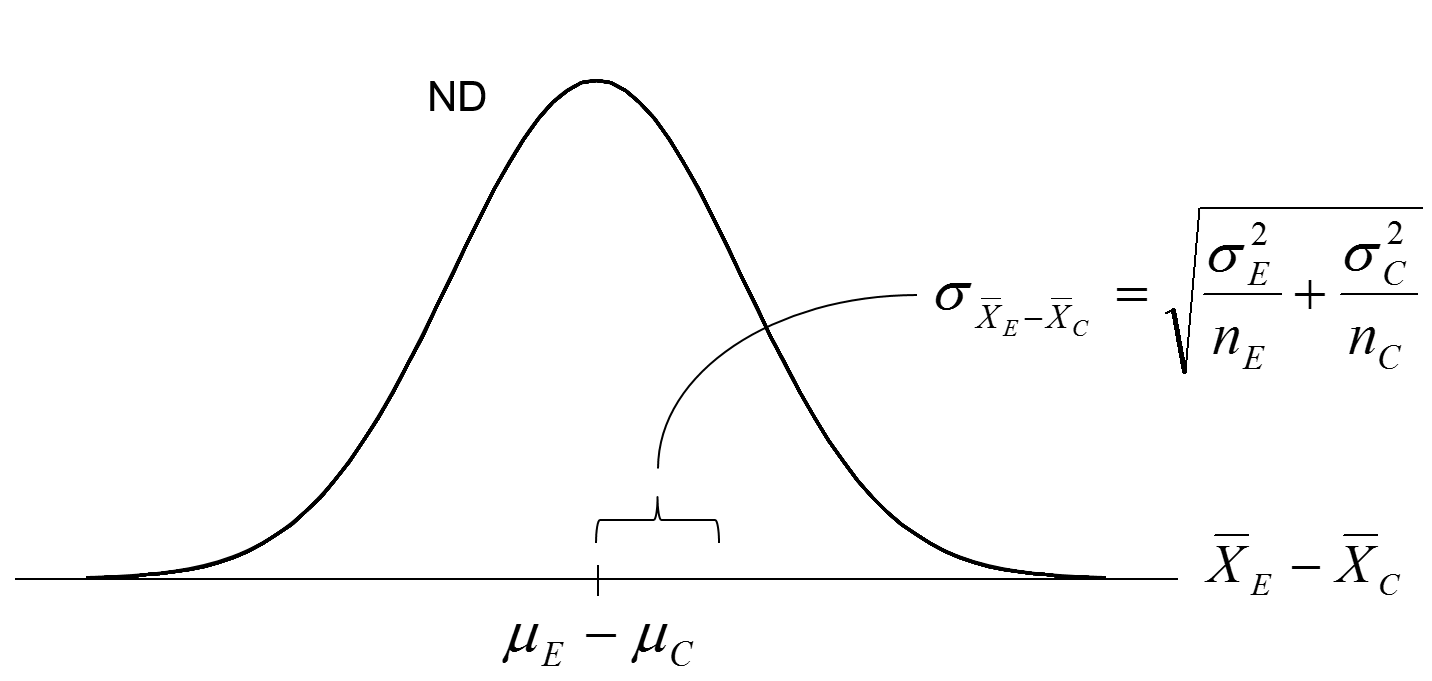
\includegraphics[width=3.5in]{samp_dist_2samp.png}
\end{itemize}

\section{Example 1 (cont.)}\label{example-1-cont.-1}

\[ \sigma_{\bar{X}_{E} - \bar{X}_{C}} = \sqrt{\frac{\sigma_{E}^{2}}{n_{E}} + \frac{\sigma_{C}^{2}}{n_{C}}} \]
- What is the \(Pr(\bar{X}_{E} - \bar{X}_{C} \geq 4)\)?
\[ z = \frac{(\bar{X}_{E} - \bar{X}_{C}) - (\mu_{E} - \mu_{C})_{HYP}}{\sigma_{\bar{X}_{E} - \bar{X}_{C}}} \]

\section{Sampling Distribution
Explanation}\label{sampling-distribution-explanation}

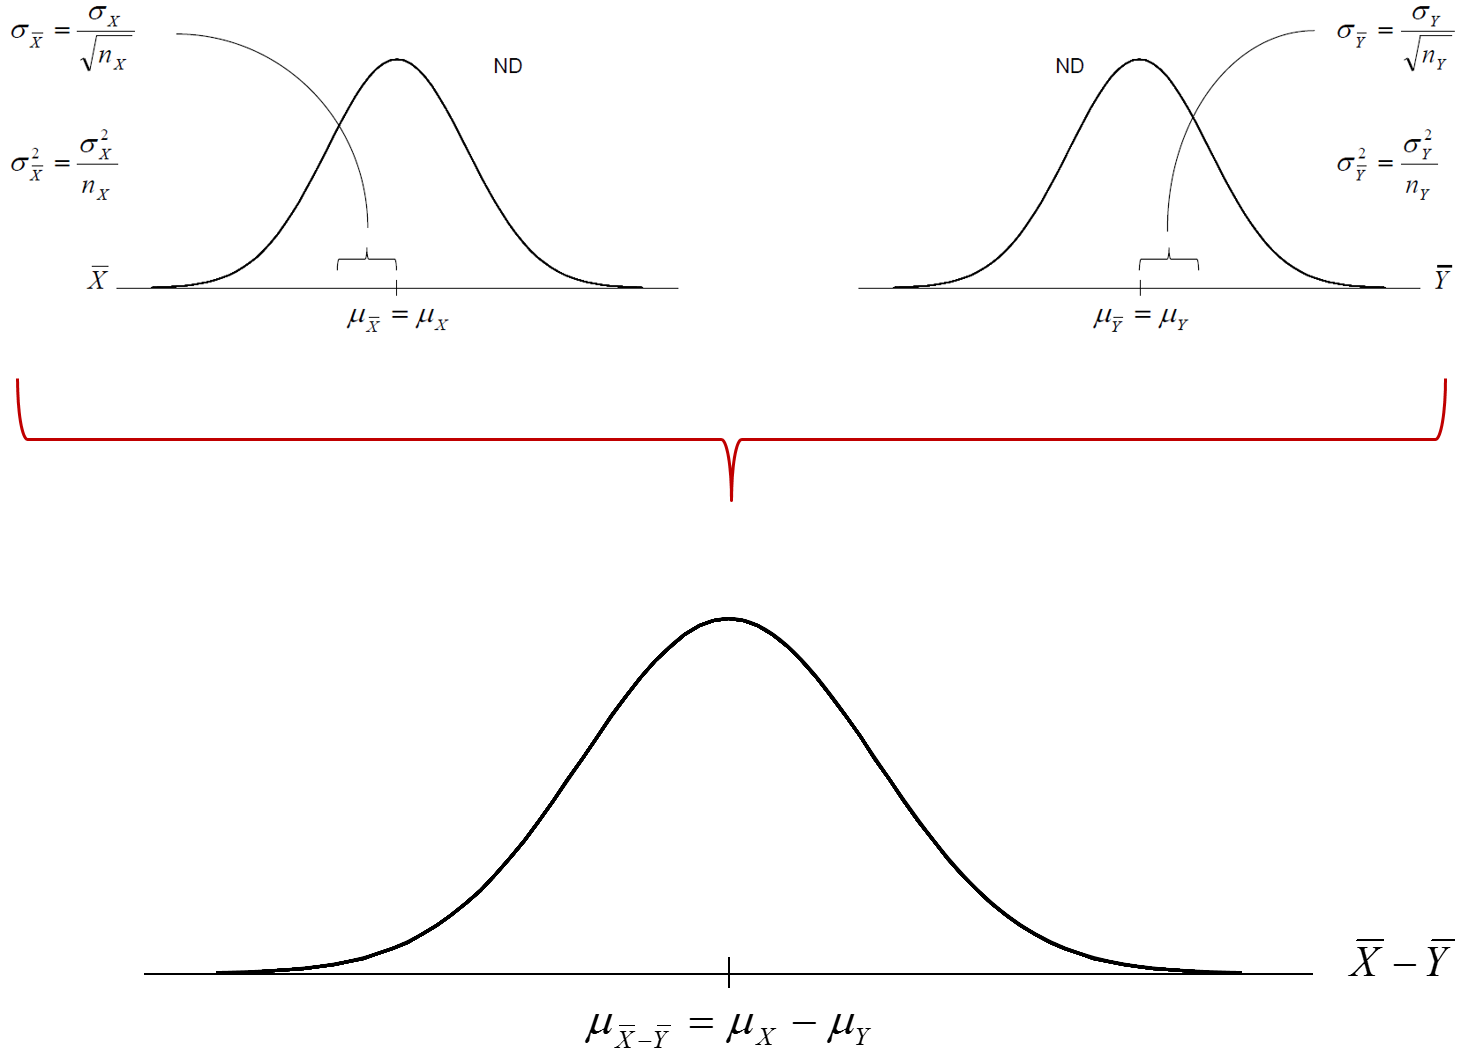
\includegraphics[width=3.5in]{samp_dist_2samp_comb.png}
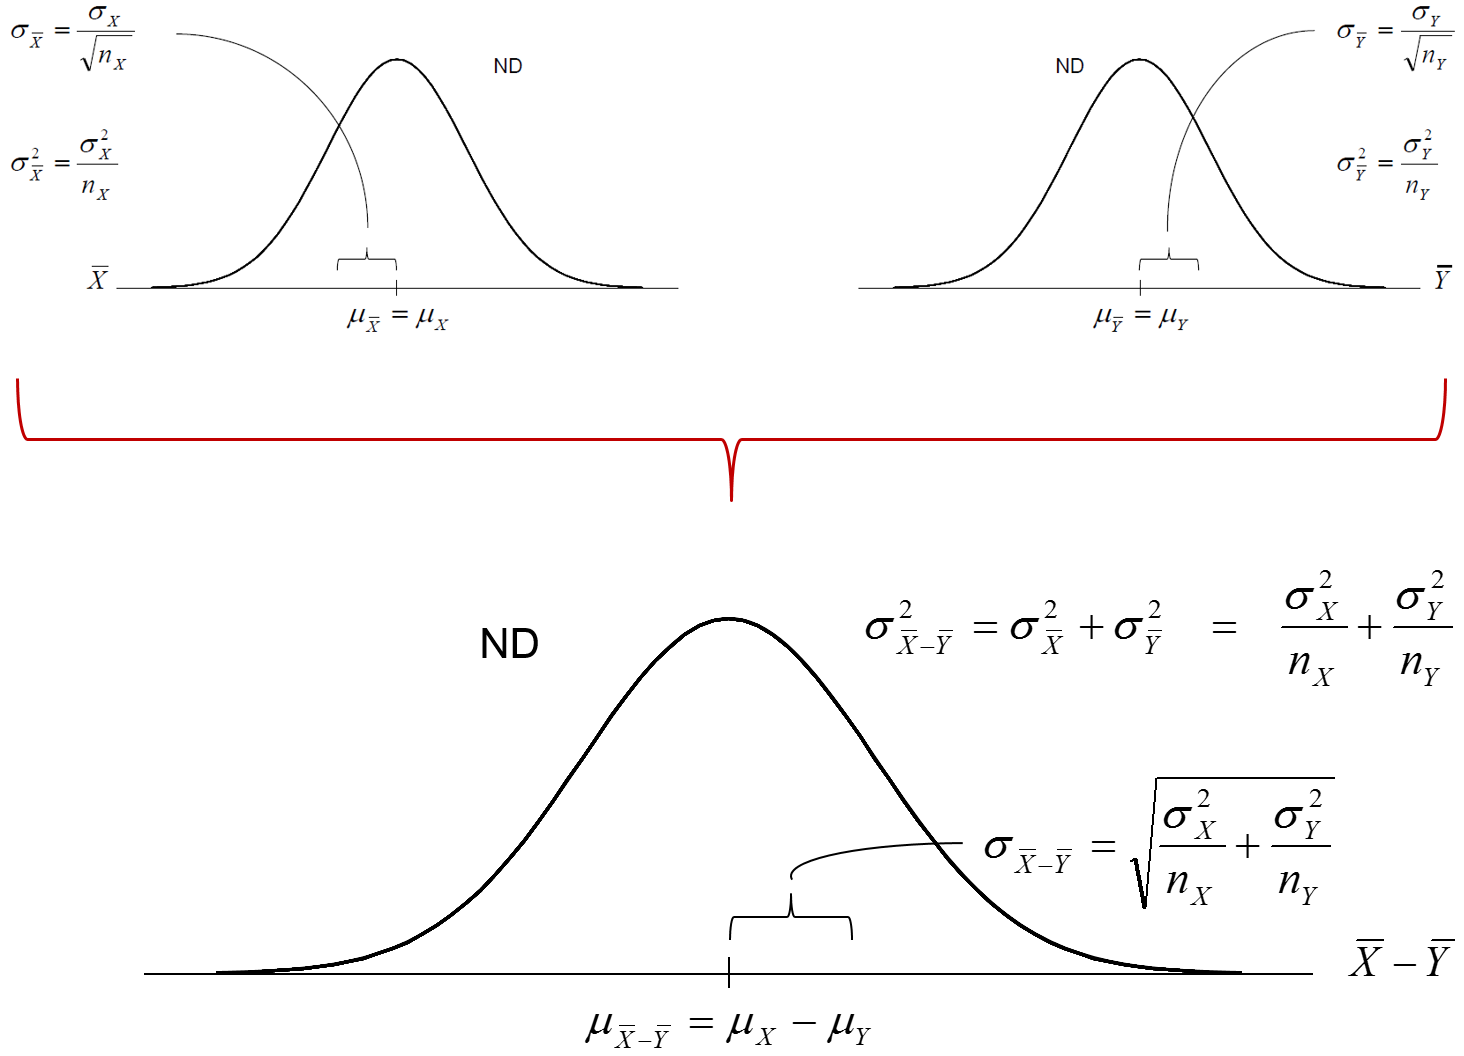
\includegraphics[width=3.5in]{samp_dist_2samp_comb_all.png}

\section{When population SDs are
unknown}\label{when-population-sds-are-unknown}

\begin{itemize}
\itemsep1pt\parskip0pt\parsep0pt
\item
  Recall:
  \(\sigma_{\bar{X} - \bar{Y}} = \sqrt{\frac{\sigma_{X}^{2}}{n_{X}} + \frac{\sigma_{Y}^{2}}{n_{Y}}}\)
\item
  Assumption: \(\sigma_{X}^{2} = \sigma^2_{X} = \sigma^2\)
\item
  Then:
  \(\sigma_{\bar{X} - \bar{Y}} = \sqrt{\frac{\sigma^{2}}{n_{X}} + \frac{\sigma^{2}}{n_{Y}}}\)
\item
  Now:
  \(\hat{\sigma}_{\bar{X} - \bar{Y}} = \sqrt{\frac{\hat{\sigma}^{2}}{n_{X}} + \frac{\hat{\sigma}^{2}}{n_{Y}}} = \sqrt{\hat{\sigma}^2\left(\frac{1}{n_{X}} + \frac{1}{n_{Y}}\right)}\)
\end{itemize}

\section{When population SDs are unknown
2}\label{when-population-sds-are-unknown-2}

\begin{itemize}
\itemsep1pt\parskip0pt\parsep0pt
\item
  \(\hat{\sigma}_{\bar{X} - \bar{Y}} = \sqrt{\frac{\hat{\sigma}^{2}}{n_{X}} + \frac{\hat{\sigma}^{2}}{n_{Y}}} = \sqrt{\hat{\sigma}^2\left(\frac{1}{n_{X}} + \frac{1}{n_{Y}}\right)}\)
\item
  \(\hat{\sigma}^2\) is a weighted average of the unbiased estimates of
  \(\sigma^2_{X}\) and \(\sigma^2_{Y}\)
\item
  Since \(\sigma^2_{X}\) and \(\sigma^2_{Y}\) are both not known to us:
  \(\hat{\sigma}_{\bar{X} - \bar{Y}} = \sqrt{\frac{n_{X}S^2_{X} + n_{Y}S^2_{Y}}{(n_{X} - 1) + (n_{Y} - 1)} \left(\frac{1}{n_{X}} + \frac{1}{n_{Y}}\right)}\)
\end{itemize}

\section{Putting all together: Pop SDs
unknown}\label{putting-all-together-pop-sds-unknown}

\begin{figure}[H]
\centering
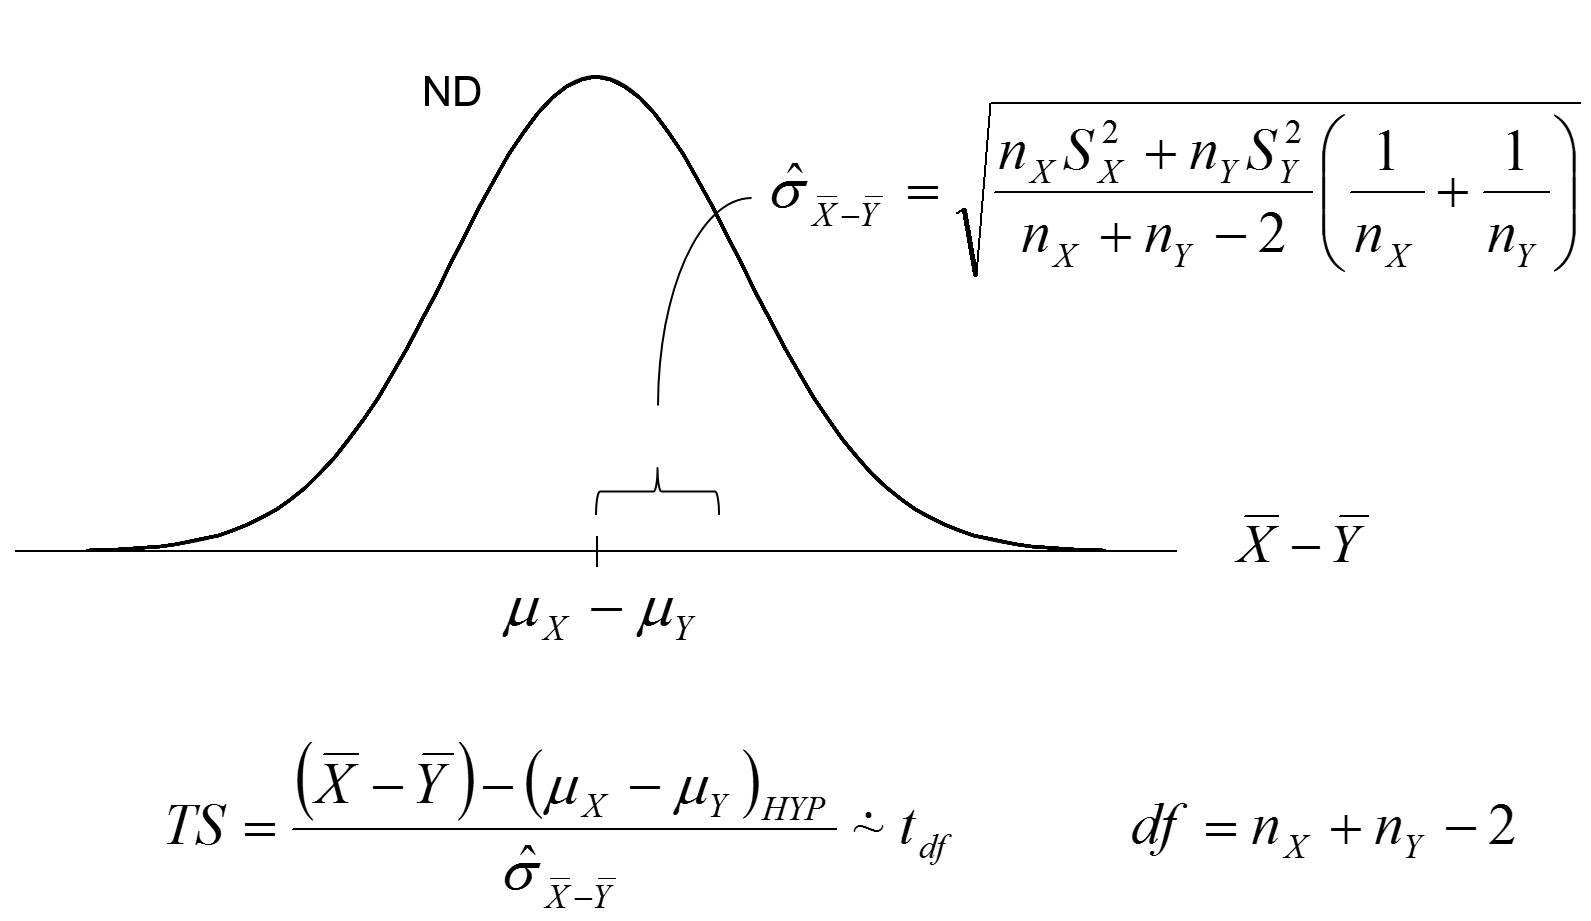
\includegraphics[width=3.5in]{samp_dist_2samp_tdist.png}
\caption{}
\end{figure}

\section{Example 2}\label{example-2}

\begin{itemize}
\itemsep1pt\parskip0pt\parsep0pt
\item
  Does speed reading help or hurt reading comprehension?
\item
  Random sample of UI freshman students, \(n = 100\)
\item
  Divide randomly in 2 groups of 50
\end{itemize}

\begin{longtable}[c]{@{}lll@{}}
\toprule
& Experimental & Control\tabularnewline
\midrule
\endhead
n & 50 & 50\tabularnewline
\(\bar{X}\) & 35 & 31\tabularnewline
\(S\) & 8 & 6\tabularnewline
\bottomrule
\end{longtable}

\begin{itemize}
\itemsep1pt\parskip0pt\parsep0pt
\item
  Conduct the hypothesis test at \(\alpha = 0.01\) significance level.
\end{itemize}

\section{Summary}\label{summary}

\begin{itemize}
\itemsep1pt\parskip0pt\parsep0pt
\item
  If Population SDs are known:
  \[ \sigma_{\bar{X} - \bar{Y}} = \sqrt{\frac{\sigma_{X}^{2}}{n_{X}} + \frac{\sigma_{Y}^{2}}{n_{Y}}} \]
  \[ TS = \frac{(\bar{X} - \bar{Y}) - (\mu_{X} - \mu_{Y})_{HYP}}{\sigma_{\bar{X} - \bar{Y}}} \sim Z \]
\item
  If Population Sds are \textbf{NOT} known:
  \[ \hat{\sigma}_{\bar{X} - \bar{Y}} = \sqrt{\frac{n_{X}S^2_{X} + n_{Y}S^2_{Y}}{(n_{X} - 1) + (n_{Y} = 1)} \left(\frac{1}{n_{X}} + \frac{1}{n_{Y}}\right)} \]
  \[ TS = \frac{(\bar{X} - \bar{Y}) - (\mu_{X} - \mu_{Y})_{HYP}}{\hat{\sigma}_{\bar{X} - \bar{Y}}} \sim t_{df} \]
  \[ df = n_{X} + n_{Y} - 2 \]
\end{itemize}

\section{Example 3}\label{example-3}

\begin{itemize}
\itemsep1pt\parskip0pt\parsep0pt
\item
  2 methods (A \& B) of teaching addition of fractions
\item
  Is method A more effective than Method B?
\item
  Randomly sample 2 classes
\item
  Results:
\end{itemize}

\begin{longtable}[c]{@{}lll@{}}
\toprule
& A & B\tabularnewline
\midrule
\endhead
n & 10 & 24\tabularnewline
\(\bar{X}\) & 115 & 105\tabularnewline
\(S\) & 14 & 17\tabularnewline
\bottomrule
\end{longtable}

\begin{itemize}
\itemsep1pt\parskip0pt\parsep0pt
\item
  Conduct the hypothesis test at the \(\alpha = .05\) significance
  level.
\end{itemize}

\section{Assumptions}\label{assumptions}

\begin{enumerate}
\def\labelenumi{\arabic{enumi}.}
\itemsep1pt\parskip0pt\parsep0pt
\item
  Each sample is drawn at random from its respective population
\item
  The two samples must be independently selected.
\item
  Sampling with replacement, or \$ n \textless{} 5\%\$ of N.
\item
  The two populations (of raw scores) are normally distributed.
\item
  The unknown population variances are equal (homogeneity of variances
  assumption).
\end{enumerate}

\section{Assumptions 1 - 3}\label{assumptions-1---3}

\begin{itemize}
\itemsep1pt\parskip0pt\parsep0pt
\item
  In Example 2, we analyzed the data as if we had drawn each of the two
  samples

  \begin{itemize}
  \itemsep1pt\parskip0pt\parsep0pt
  \item
    independent (assumption 2)
  \item
    from its respective population randomly (assumption 1)
  \item
    with replacement (assumption 3)
  \end{itemize}
\item
  However, that is not how the experiment was done.

  \begin{itemize}
  \itemsep1pt\parskip0pt\parsep0pt
  \item
    First, we randomly sampled without replacement from a single
    population
  \item
    Then, we randomly assigned each participant to one of two groups
    (experimental or control)
  \item
    This is called a randomized experiment
  \end{itemize}
\end{itemize}

\section{Assumptions 1 - 3 (cont)}\label{assumptions-1---3-cont}

\begin{itemize}
\itemsep1pt\parskip0pt\parsep0pt
\item
  In other words, a random sampling model (Independent Means t-Test) was
  used to analyze data that came from two groups formed by random
  assignment
\item
  Technically, a random assignment model (Permutation Test) should have
  been used to analyze the data
\item
  Two mistakes when analyzing the data as we did

  \begin{enumerate}
  \def\labelenumi{\arabic{enumi}.}
  \itemsep1pt\parskip0pt\parsep0pt
  \item
    Draws were made without replacement (inflates the SE)
  \item
    There was a slight degree of dependency between the two groups
    (deflates the SE)
  \end{enumerate}
\end{itemize}

\section{Assumptions 1 - 3 (cont)}\label{assumptions-1---3-cont-1}

\begin{itemize}
\itemsep1pt\parskip0pt\parsep0pt
\item
  It is a lucky break that in randomized experiments, the first mistake
  outweighs the second

  \begin{itemize}
  \itemsep1pt\parskip0pt\parsep0pt
  \item
    Thus, when the random sampling model is applied to randomized
    experiments, the statistical test is conservative (the SE tends to
    be overestimated)
  \end{itemize}
\item
  For most randomized experiments, using the random sampling model
  yields the same statistical conclusions as the random assignment model
\item
  However, with only random assignment of available participants,
  conclusions do not generalize beyond

  \begin{itemize}
  \itemsep1pt\parskip0pt\parsep0pt
  \item
    the participants studied, and
  \item
    the conditions of the study
  \end{itemize}
\end{itemize}

\section{Random Sampling vs Random
Assignment}\label{random-sampling-vs-random-assignment}

\begin{itemize}
\itemsep1pt\parskip0pt\parsep0pt
\item
  Random Sampling

  \begin{itemize}
  \itemsep1pt\parskip0pt\parsep0pt
  \item
    a method for obtaining a sample from an experimentally accessible
    population
  \item
    a basic assumption underlying statistical inference
  \item
    this is what makes it possible for us to make statistical
    conclusions based on theoretical probability models, and generalize
    those conclusions to a population
  \end{itemize}
\item
  Random Assignment

  \begin{itemize}
  \itemsep1pt\parskip0pt\parsep0pt
  \item
    a method for dividing an available group of participants into two or
    more subgroups
  \item
    its purpose is to make the comparison groups randomly equivalent to
    each other prior to any treatment(s)
  \item
    it controls for extraneous variables (known and unknown)
  \end{itemize}
\end{itemize}

\section{The normality assumption}\label{the-normality-assumption}

\begin{itemize}
\itemsep1pt\parskip0pt\parsep0pt
\item
  The independent means t-test is robust with respect to violations of
  the normality assumption

  \begin{itemize}
  \itemsep1pt\parskip0pt\parsep0pt
  \item
    If the two sample sizes are equal, the t-test gives fairly accurate
    p-values for a broad range of population distributions, provided the
    populations

    \begin{itemize}
    \itemsep1pt\parskip0pt\parsep0pt
    \item
      have similar shapes
    \item
      are unimodal
    \item
      have no outliers
    \end{itemize}
  \item
    This holds for sample sizes as small as \(n_{X} = n_{Y} = 5\)
  \end{itemize}
\item
  When \(n_{X}\) and \(n_{Y}\) are both greater than 30, the normality
  assumption is unimportant, thanks to the central limit theorem
\end{itemize}

\section{The homogeneity of variance
assumption}\label{the-homogeneity-of-variance-assumption}

\begin{itemize}
\itemsep1pt\parskip0pt\parsep0pt
\item
  The independent means t-test is robust with respect to violations of
  the assumption of equal population variances, provided that
  \(n_{X} = n_{Y}\)
\item
  There is a statistical test of the equality of population variances

  \begin{itemize}
  \itemsep1pt\parskip0pt\parsep0pt
  \item
    F-test
  \end{itemize}
\item
  If the population variances are unequal, and if \(n_{X} \neq n_{Y}\),
  the sample variances should not be pooled

  \begin{itemize}
  \itemsep1pt\parskip0pt\parsep0pt
  \item
    A modified t-statistic with modified df can be used, often times
    called the Welch t-test
  \end{itemize}
\end{itemize}

\section{Confidence Intervals}\label{confidence-intervals}

\begin{itemize}
\itemsep1pt\parskip0pt\parsep0pt
\item
  Recall the speed reading data:
\end{itemize}

\begin{longtable}[c]{@{}lll@{}}
\toprule
& Experimental & Control\tabularnewline
\midrule
\endhead
n & 50 & 50\tabularnewline
\(\bar{X}\) & 35 & 31\tabularnewline
\(S\) & 8 & 6\tabularnewline
\bottomrule
\end{longtable}

\begin{itemize}
\itemsep1pt\parskip0pt\parsep0pt
\item
  Find a 99\% CI for \(\mu_{E} - \mu_{C}\)
\item
  Confidence form looks as follows:
  \[ (\bar{X} - \bar{X}) \pm t_{crit} \hat{\sigma}_{\bar{X} - \bar{Y}} \]
\end{itemize}

\section{Confidence Interval
Interpretations}\label{confidence-interval-interpretations}

\begin{itemize}
\itemsep1pt\parskip0pt\parsep0pt
\item
  Interpretations for 99\% CI {[}0.24, 7.76{]}:

  \begin{enumerate}
  \def\labelenumi{\arabic{enumi}.}
  \itemsep1pt\parskip0pt\parsep0pt
  \item
    Does \(\mu\) fall in this interval?
  \item
    Is there a 99\% chance that \(\mu\) falls in this interval?
  \item
    If 100 intervals were constructed, about how many intervals would
    contain \(\mu\)?
  \item
    If we constructed an infinte number of intervals, how many would
    contain \(\mu\)?
  \end{enumerate}
\end{itemize}

\section{Using confidence intervals to conduct a two-tailed
hypothesis}\label{using-confidence-intervals-to-conduct-a-two-tailed-hypothesis}

\begin{itemize}
\itemsep1pt\parskip0pt\parsep0pt
\item
  You can use a confidence interval to conduct a two-tailed hypothesis
  of any null hypothesis.

  \begin{itemize}
  \itemsep1pt\parskip0pt\parsep0pt
  \item
    If the hypothesized value falls within the CI, fail to reject
    \(H_{0}\)
  \item
    If the hypothesized value falls outside the CI, reject \(H_{0}\)
  \end{itemize}
\item
  Using the previous example {[}0.24, 7.76{]}, would we fail to reject
  or reject \(H_{0}\)?
\end{itemize}

\end{document}
